\documentclass[]{exam}

\usepackage{amsmath}
\usepackage{amsthm}
\usepackage{graphicx}
\usepackage{subcaption}

\pagestyle{empty}

\begin{document}
  \begin{center}
    \fbox{\fbox{\parbox{5.5in}{\centering Answer the questions in the spaces
    provided on the question sheets. If you run out of room for an answer,
    continue on a separate sheet of paper.}}}
  \end{center}

  \section*{Product and sum rule}

  Consider the following definitions for sets of characters:

  \begin{itemize}
    \item Digits = $\{\ 0\ ..\ 9\ \}$
    \item Letters = $\{\ a\ ..\ z\ \}$
    \item Special characters = $\{\ *,\ \&,\ \$,\ \#\ \}$
  \end{itemize}

  \begin{questions}
    \question Compute the number of passwords that satisfy the given
    constraints.
      \begin{parts}
        \part Strings of length 6. Characters can be special characters, digits,
          or letters.
          \begin{solution}
            Let $D$ be the set of digits, $L$ the set of letters, and $S$ the
            set of special characters. The three sets are mutually disjoint, so
            the total number of characters is

            \bigskip

            $|D \cup L \cup S| = |D| + |L| + |S| = 10 + 26 + 4 = 40$

            \bigskip

            Each of the six characters in the string can be any of the 40
            characters, so there are a total of $40^6$ strings of length 6.
          \end{solution}
          \vspace{\stretch{1}}

        \part Strings of length 7, 8, or 9. Characters can be special
          characters, digits, or letters.
          \begin{solution}
            The sets of strings of length 7, 8, and 9 are mutually disjoint. The
            number of strings of length $j$ with no other restrictions on the
            characters is $40^j$. Therefore, by the sum rule, the total number
            of strings of length 7, 8, or 9 is:

            \bigskip

            $40^7 + 40^8 + 40^9$
          \end{solution}
          \vspace{\stretch{1}}

        \part Strings of length 7, 8, or 9. Characters can be special
          characters, digits, or letters. The first character cannot be a
          letter.
          \begin{solution}
            In selecting a string of length $j$ in which the first character is
            not a letter, there are 14 choices for the first character because
            there are $4 + 10$ digits and special characters. There are 40
            choices for each of the remaining characters. Putting the choices
            together by the product rule, the total number of strings of length
            $j$ in which the first character is not a letter is
            $14\cdot40^{j-1}$. Sets of strings of length 7, 8, and 9 are
            mutually disjoint. Therefore, by the sum rule, the number of strings
            of length 7, 8, or 9 which do not start with a letter is:

            \bigskip

            $14\cdot40^6 + 14\cdot40^7 + 14\cdot40^8 = 14(40^6 + 40^7 + 40^8)$
          \end{solution}
          \vspace{\stretch{1}}
      \end{parts}

    \question Consider the numbers in the range 1 to $10^4$ (inclusive).
      \begin{parts}
        \part How many of the numbers in the range $10^3$ to $10^4$ (inclusive)
          are composed of all distinct digits?
          \begin{solution}
            By the generalized product rule, $9\cdot9\cdot8\cdot7=4536$ numbers
            are composed of distinct digits. \emph{Note: the first digit cannot
            be zero, thus this initial 9 factor.} $10^4$ has repeated digits, so
            we don't count it.
          \end{solution}
          \vspace{\stretch{1}}

        \part How many of the numbers in the range 1 to $10^4$ (inclusive) are
          composed of all distinct digits?
          \begin{solution}
            9 single digit numbers, $9\cdot 9=81$ two digit numbers,
            $9\cdot9\cdot8=648$ three digits numbers, and 4536 four digit
            numbers.

            \bigskip

            $9 + 81 + 648 + 4536=5274$
          \end{solution}
          \vspace{\stretch{1}}
      \end{parts}

    %\uplevel{\section*{Bijection rule}}

    \newpage

    \uplevel{
      \section*{Permuations}

      Consider the following permutations of a single adjacency matrix:
    }

    \begin{figure}[h!]
      \centering
      \begin{subfigure}[b]{0.3\textwidth}
        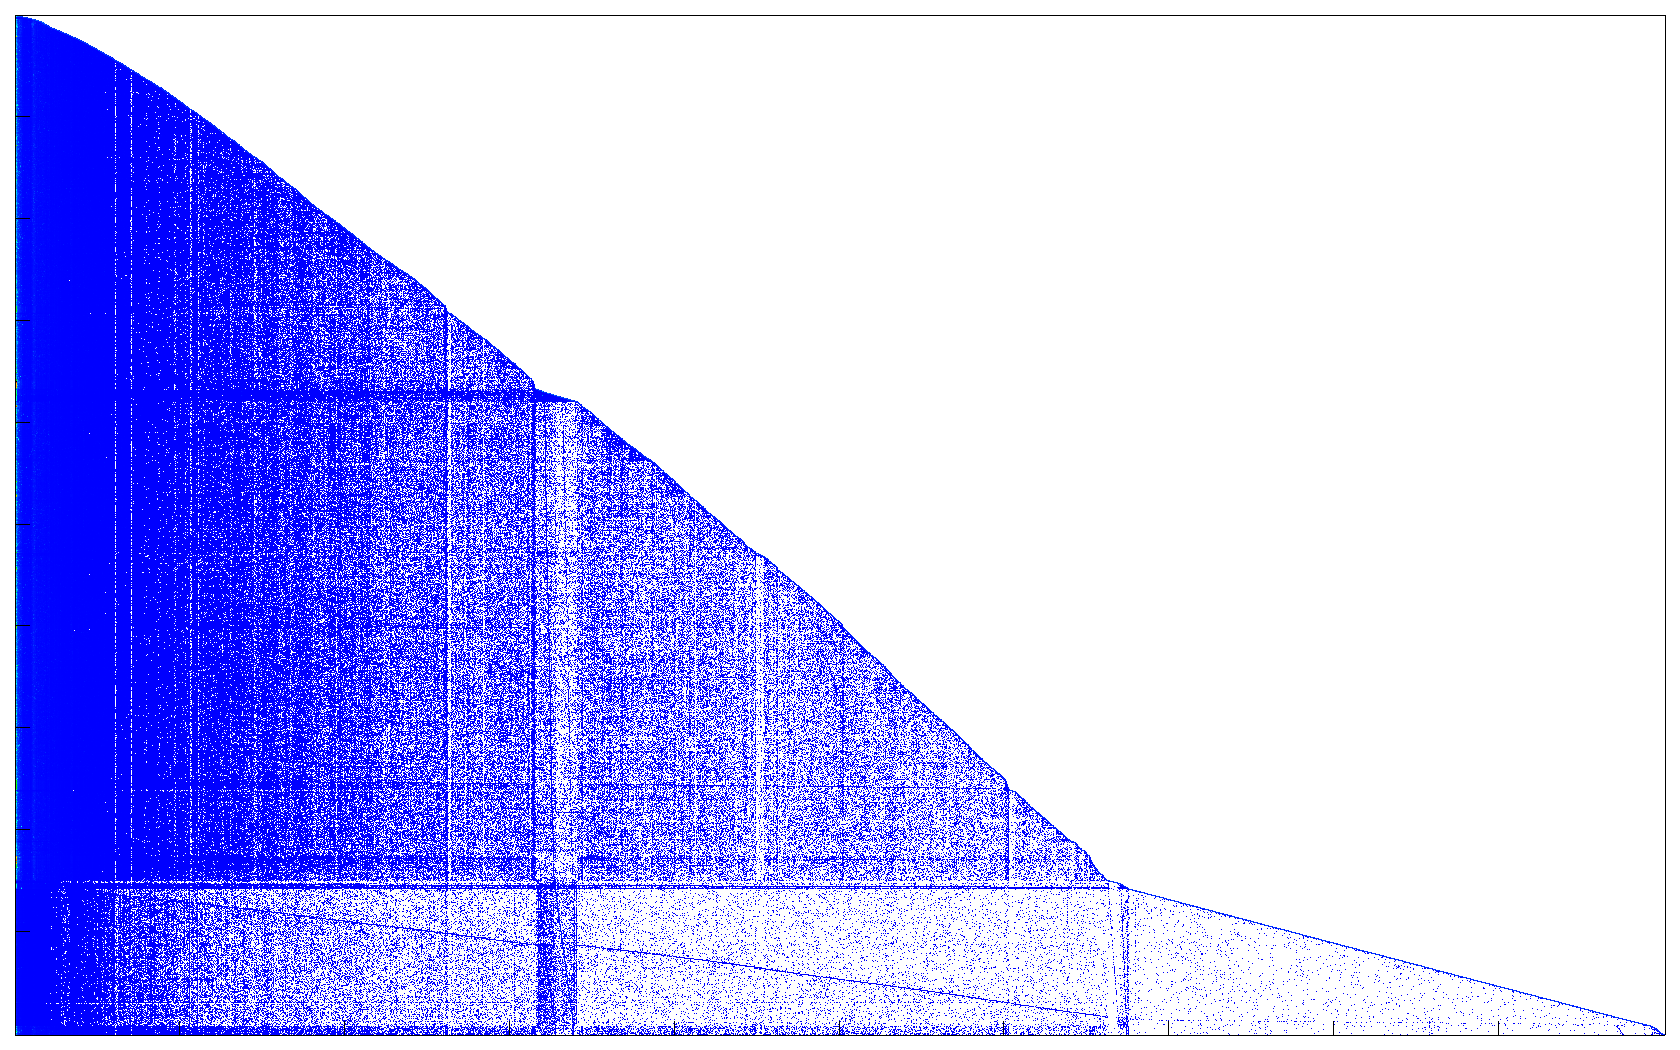
\includegraphics[width=\textwidth]{orig}
        \caption{Original}
      \end{subfigure}
      ~
      \begin{subfigure}[b]{0.3\textwidth}
        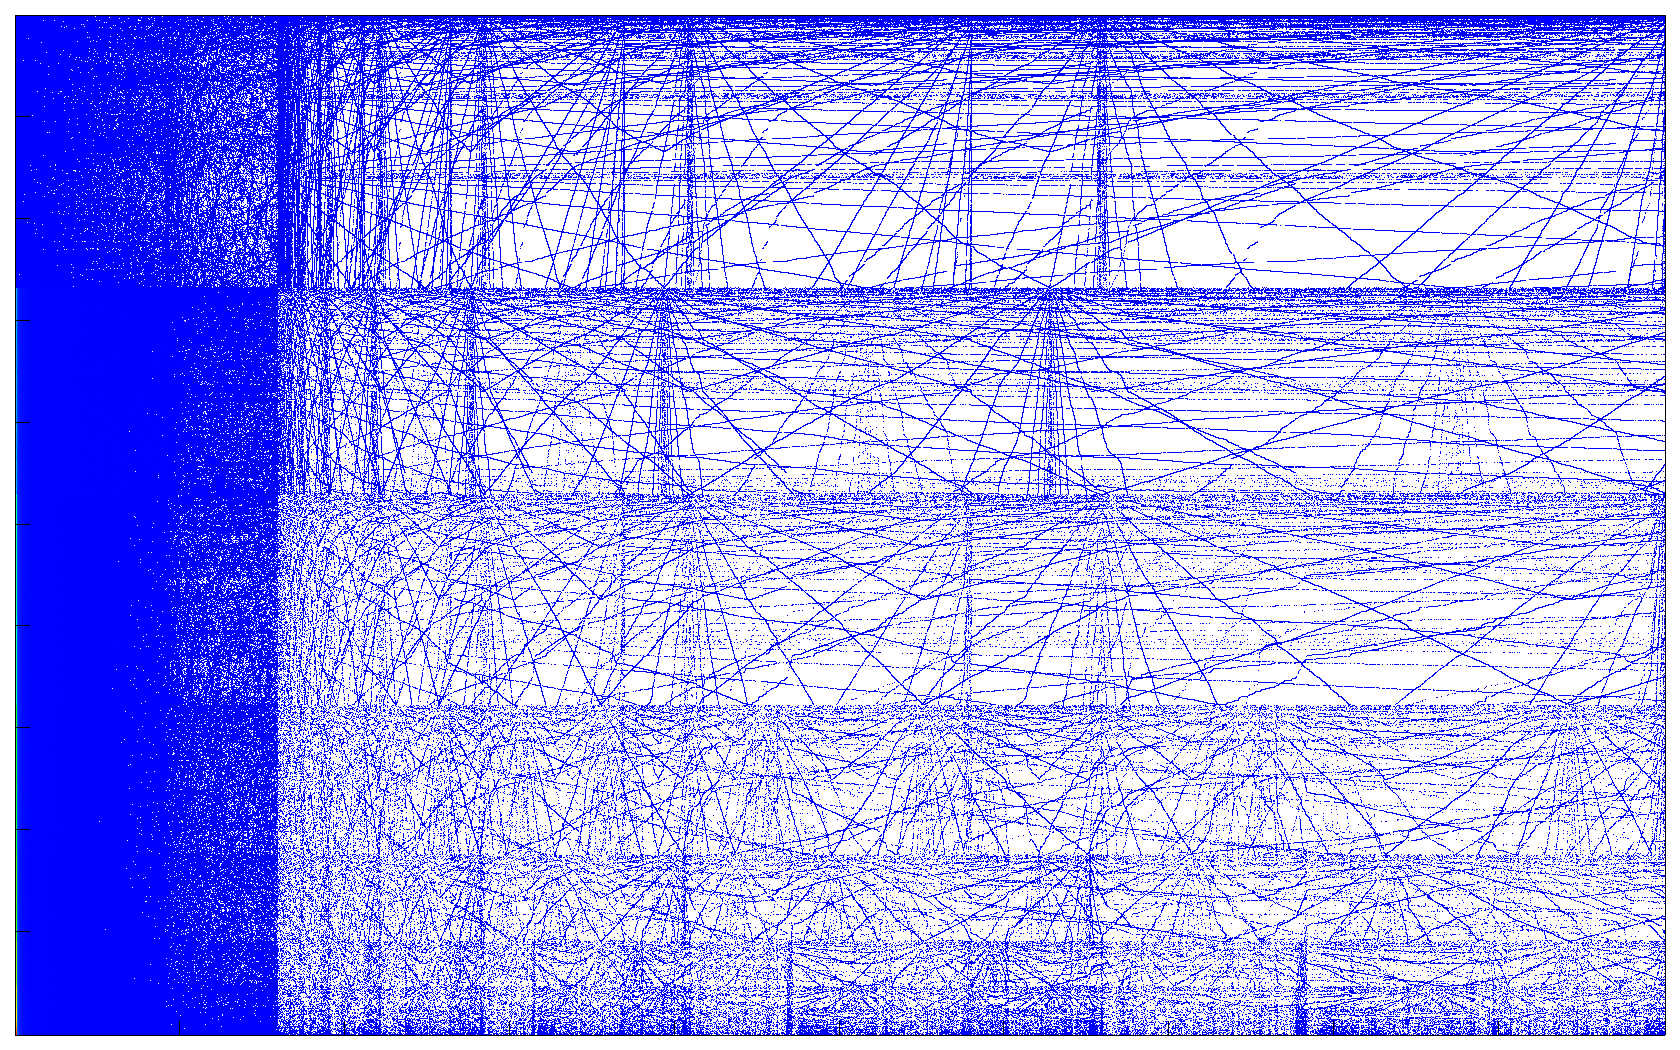
\includegraphics[width=\textwidth]{clean}
        \caption{Clean}
      \end{subfigure}
      ~
      \begin{subfigure}[b]{0.3\textwidth}
        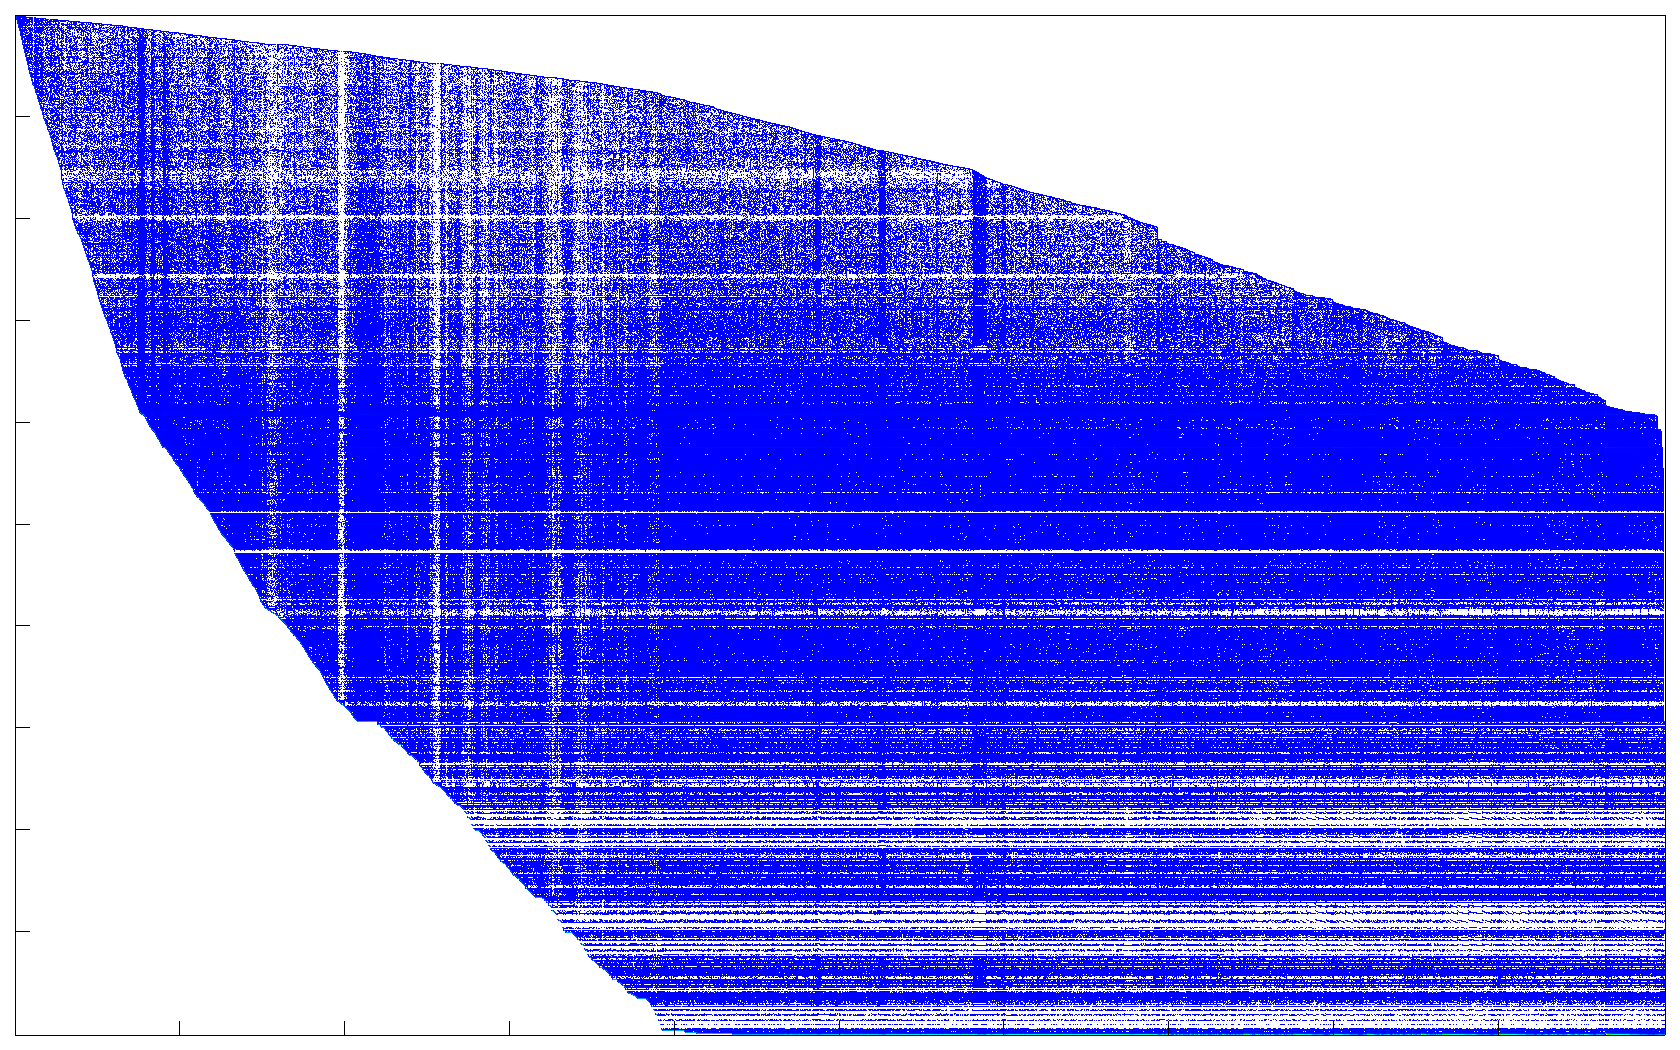
\includegraphics[width=\textwidth]{rcm}
        \caption{RCM}
      \end{subfigure}
    \end{figure}

    Permuting the rows / columns of a matrix can be beneficial for a couple
    reasons:

      \begin{enumerate}
        \item Improve computational efficiency by improving structure of
          adjacency matrix
        \item Expose hidden structure in the graph
      \end{enumerate}

    Unfortunately, knowing \emph{apriori} which permutation is best is a
    difficult problem. The problem is compounded by the huge number of
    permutations possible.

    As a result, \emph{heuristic} methods are usually employed. These methods,
    like (b) and (c) above, are efficient to find and lead to good, but not
    necessarily optimal, permutations of the matrix.

    \bigskip

    \question How many ways are there to permute the rows / columns of a
      \begin{parts}
        \part $10\times10$ matrix?
          \begin{solution}
            $10!=3628800$
          \end{solution}
          \vspace{\stretch{1}}
        \part $n\times n$ matrix?
          \begin{solution}
            $n!$
          \end{solution}
          \vspace{\stretch{1}}
      \end{parts}

    \uplevel{\section*{Combinations}}

    \question Suppose a network has 40 computers of which 5 fail.
      \begin{parts}
        \part How many possibilities are there for the five that fail?
          \begin{solution}
            $\binom{40}{5}=\frac{40!}{5!(40-5)!}=\frac{40\cdot39\cdot38\cdot37\cdot36}{5\cdot4\cdot3\cdot2\cdot1}=658008$
          \end{solution}
          \vspace{\stretch{1}}

        \part Suppose that 3 of the computers in the network have a copy of a
          particular file. How many sets of failures wipe out all the copies of
          the file? That is, how many 5-subsets contain the three computers that
          have the file?
          \begin{solution}
            Any such 5-subset of computers that fail must contain the 3
            computers that have the file. The two remaining computers in the
            subset must be selected from the 37 computers that did not contain
            the file. Thus, the number of such 5-subsets in which the 3
            computers with the file fail is the number of ways to select 2
            computers from the 37 computers without the file, or
            $\binom{37}{2}$. 
          \end{solution}
          \vspace{\stretch{1}}
      \end{parts}
  \end{questions}
\end{document}
